
\setcounter{chapter}{4}
\setcounter{section}{0}
\setcounter{figure}{0}
\setcounter{table}{0}
\chapter* {\begin{flushleft}
CHƯƠNG 4\\
\end{flushleft}LẬP TRÌNH GIAO DIỆN ĐỒ HỌA} 
\addcontentsline{toc}{chapter}{Chương 4. XPath - XQuery - XLink - XPointer}
%\thispagestyle{fancy}
Ngoài ứng dụng độc lập (console Application), Java cho phép  xây dựng các ứng dụng có giao diện đồ hoạ (Grapthical User Interface: GUI). Đầu tiên, Java hỗ trợ các thành phần đồ hoạ được tập trung vào thư viện mang tên Abstract Window
Toolkit (AWT), sau đó kế thừa lên AWT Java xây dựng thư viên Swing.




Đối với mỗi hệ nền, thành phần AWT sẽ được ánh xạ sang một
thành phần nền cụ thể, bằng cách sử dụng trực tiếp mã native của hệ nền, chính vì
vậy nó phụ thuộc rất nhiều vào hệ nền và nó còn gây lỗi trên một số hệ nền. Với
bản phát hành Java 2, các thành phần giao diện được thay bằng tập hợp các thành
phần linh hoạt, đa năng, mạnh mẽ, độc lập với hệ nền thuộc thư viện Swing. Phần
lớn các thành phần trong thư viện Swing đều được tô vẽ trược tiếp trên canvas
bằng mã lệnh của Java, ngoại trừ các thành phần là lớp con của lớp
java.awt.Window hoặc Java.awt.Panel vốn phải đựơc vẽ bằng GUI trên nền cụ thể.
Thành phần Swing ít phụ thuộc vào hệ nền hơn do vậy ít gặp lỗi hơn và đặc biệt
nó sử dụng ít tài nguyên của hệ thống hơn các thành phần trong thư viện awt. Mặc
dù các thành phần awt vẫn được hỗ trợ trong Java 2 nhưng, tuy nhiên Sun khuyên
bạn nên sử dụng các thành phần Swing thay cho các thành phần awt, tuy nhiên các
thành phần trong thư viện Swing không thể thay tất cả các thành phần trong thư
viện awt. Chúng chỉ thay thế một phần của awt như: Button, Panel, TextFeild, v.v.
Còn các lớp trợ giúp khác trong awt như : Graphics, Color, Font, FontMetrics, v.v.
vẫn không thay đổi. Bên cạnh đó các thành phần Swing còn sử dụng mô hình xử lý
sự kiện của awt
\section{Giới thiệu về hệ thống đồ hoạ của Java}
Thiết kế API cho lập trình đồ hoạ của Java là một ví dụ hoàn hảo về cách dùnglớp, sự kế thừa và giao diện. API cho lập trình độ hoạ bao gồm một tập rất nhiều
lớp nhằm trợ giúp xây dựng các thành phần giao diện khác nhau như: cửa sổ,nút
ấn, ô văn bản, menu, hộp kiểm, v.v. Mối quan hệ kế thừa giữa các thành phần này
được mô tả trong hình sau:
\begin{enumerate}
	\item Componient Đây là lớp (trừu tượng) cha của mọi lớp giao diện người dùng.
Lớp này cung cấp các thuộc tính, hành vi cơ bản nhất của tất cả các thành
phần giao diện.
	\item  Container Là một vật chứa dùng để ghép nhóm các thành phần giao diện
khác. Mỗi vật chứa có một lớp quản lý hiển thị, lớp quản lý hiển thị có
trách nhiệm bố trí cách thức hiển thị các thành phần bên trong. Hai vật chứa
hay được sử dụng nhất la JFrame và JPanel.
	\item  Jcomponient Là lớp cha của mọi thành phần Swing ligth weight, được vẽ
trực tiếp lên canvas bằng mã lệnh Java.
	\item  Window Được sử dụng để tạo ra một cửa sổ, Thông thường ta hay sử dụng
hai lớp con của nó là JFrame và JDialog.
	\item  JFrame là cửa sổ không lồng bên trong cửa sổ khác.
	\item  JDialog là một cửa sổ được hiển thị dưới dạng modal.
	\item  JAplet là lớp cha của mọi lớp ứng dụng aplet.
	\item  JPanel là một vật chứa, lưu giữ các thành phần giao diện người dùng.
	\item  Graphics là lớp trừu tượng cung cấp ngữ cảnh đồ hoạ để vẽ các đối tượng
đồ hoạ như: Đường thẳng, đường tròn, hình ảnh…
	\item  Color lớp này biểu diễn một mầu sắc.
	\item  Font lớp này biểu thị cho một font đồ hoạ.
	\item  FontMetrics là một lớp trừu tượng dùng để xác định các thuộc tính của
Font.
\end{enumerate}

Tất cả các thành phần đồ hoạ trong thư viện Swing được nhóm trong gói
javax.swing. Đa số các thành phần trong thư viện Swing đều có tiếp đầu ngữ là ‘J’,
Ví dụ một nút lệnh trong thư viện Swing có tên là JButton, một memu có tên là JMenu
\subsection{Một số phương thức của lớp Component}
Lớp Component cung cấp các thuộc tính, phương thức chung cho các lớp
con của nó. Sau đây là một số phương thức của lớp Component :
- Dimension getSize():cho lại đối tượng thuộc lớp Dimension gồm width (chiều
rộng), height (chiều cao) xác định kích thước của một thành phần tính theo pixel.
- void setSize(int width, int height) và void setSize(Dimension d) đặt lại kích
thước của thành phần.
- Point getLocation(): cho lại tọa độ (kiểu Point) trên cùng bên trái (tọa độ gốc)
của thành phần đang xét.
- void setLocation(int x, int y) và void setLocation(Point p) đặt lại các tọa độ được
chỉ định cho một thành phần.
- Rectangle getBounds():cho lại đường biên là hình chữ nhật Rectangle bao gồm
tọa độ gốc và chiều dài, chiều rộng của hình chữ nhật.
- void setBounds(int x, int y) và void setBounds(Rectangle r):đặt lại đường biên
cho một thành phần.
- void setForeground(Color c):được sử dụng để đặt màu vẽ cho thành phần đồ họa
- void setBackground(Color c):đặt màu nền cho thành phần đồ họa. Các tham số
của hai hàm này là đối tượng của lớp Color sẽ được giới thiệu ở phần sau.
- Font getFont(): được sử dụng để biết được font của các chữ đang xử lý trong
thành phần đồ họa.
- void setFont(Font f):đặt lại font chữ cho một thành phần.
- void setEnabled(boolean b):Nếu đối số b của hàm getEnabled() là true thì thành
phần đang xét hoạt động bình thường, nghĩa là có khả năng kích hoạt (enable), có
thể trả lời các yêu cầu của người sử dụng và sinh ra các sự kiện như mong muốn.
Ngược lại, nếu là false thì thành phần tương ứng sẽ không kích hoạt được, nghĩa là
không thể trả lời được các yêu cầu của người sử dụng.
- Lưu ý: Tất cả các thành phần giao diện khi khởi tạo đều được kích hoạt
- void setVisible(boolean b):Một thành phần đồ họa có thể được hiển thị lên màn
hình (nhìn thấy được) hoặc bị che giấu tùy thuộc vào đối số của hàm setVisible()
là true hay false.
\subsection{ Lớp Container}
Lớp Container là lớp con của lớp trừu tượng Component. Các lớp chứa (lớp
con của Container) cung cấp tất cả các chức năng để xây dựng các giao diện đồ
họa ứng dụng, trong đó có phương thức add() được nạp chồng dùng để bổ sung
một thành phần vào vật chứa và phương thức remove() cũng được nạp chồng để
gỡ bỏ một thành phần ra khỏi vật chứa
 \subsection{ Tạo ra Frame}
Lớp JFrame là lớp con của lớp Frame (Frame là lớp con của lớp Window)
được sử dụng để tạo ra những cửa sổ cho các giao diện ứng dụng GUI.
Kịch bản chung để tạo ra một cửa sổ là:
1. Tạo ra một frame có tiêu đề gì đó, ví dụ “My Frame” :
JFrame myWindow= new JFrame(“My Frame”);
2. Xây dựng một cấu trúc phân cấp các thành phần bằng cách sử dụng hàm
myWindow.getContentPane().add() để bổ sung thêm JPanel hoặc những
thành phần giao diện khác vào Frame:
Ví dụ: myWindow.getContentPane().add(new JButton(“OK”));// Đưa vào
một nút (JButton) có tên “OK” vào frame
3. Đặt lại kích thước cho frame sử dụng hàm setSize():
myWindow.setSize(200, 300);// Đặt lại khung frame là 200 ( 300
4. Gói khung frame đó lại bằng hàm pack():
myWindow.pack();
5. Cho hiện frame:
myWindow.setVisible(true);
\section{Trình quản lý hiển thị trong Java}
Khi thiết kế giao diện đồ họa cho một ứng dụng, chúng ta phải quan tâm
đến kích thước và cách bố trí (layout) các thành phần giao diện như: JButton,
JCheckbox, JTextField, v.v. sao cho tiện lợi nhất đối với người sử dụng. Java có
các lớp đảm nhiệm những công việc trên và quản lý các thành phần giao diện GUI
bên trong các vật chứa.
Bảng sau cung cấp bốn lớp quản lý layout (cách bố trí và sắp xếp) các thành phần
GUI.

\begin{center}
	\begin{longtable}{|m{3cm}|m{9cm}|}
		\caption[Các chế độ hiển thị]{Các chế độ hiển thị}
		\label{bang32*}
		\endfirsthead
		\endhead
		\hline
		\multicolumn{1}{|c|}{\textbf{Tên lớp}} &\multicolumn{1}{c|}{	\textbf{ Mô tả}}
		\\ \hline
	
 
FlowLayout  &Xếp các thành phần giao diện trước tiên theo hàng từ trái qua phải,
sau đó theo cột từ trên xuống dưới. Cách sắp xếp này là mặc định
đối với Panel, JPanel ,Applet và JApplet. \\ \hline
GridLayout & Các thành phần giao diện được sắp xếp trong các ô lưới hình chữ
nhật lần lượt theo hàng từ trái qua phải và theo cột từ trên xuống
dưới trong một phần tử chứa. Mỗi thành phần giao diện chứa trong
một ô. \\ \hline
BorderLayout & Các thành phần giao diện (ít hơn 5) được đặt vào các vị trí theo các
hướng: north (bắc), south (nam), west (tây), east (đông) và center
(trung tâm)). Cách sắp xếp này là mặc định đối với lớp Window,
Frame, Jframe, Dialog và JDialog. \\ \hline
GridBagLayout & Cho phép đặt các thành phần giao diện vào lưới hình chữ nhật,
nhưng một thành phần có thể chiếm nhiều nhiều hơn một ô.  \\ \hline
null & Các thành phần bên trong vật chứa không được sẵp lại khi kích
thước của vật chứa thay đổi.
		\\ \hline 
\end{longtable}
\end{center}
Các phương pháp thiết đặt layout
Để lấy về layout hay để đặt lại layout cho vật chứa, chúng ta có thể sử dụng hai
phương thức của lớp Container:
LayoutManager getLayout();
void setLayout(LayoutManager mgr);
Các thành phần giao diện sau khi đã được tạo ra thì phải được đưa vào một phần
tử chứa nào đó. Hàm add() của lớp Container được nạp chồng để thực hiện nhiệm
vụ đưa các thành phần vào phần tử chứa.
Component add(Component comp)
Component add(Component comp, int index)
Cmponent add(Component comp, Object constraints)
Cmponent add(Component comp, Object constraints, int index)
Trong đó, đối số index được sử dụng để chỉ ra vị trí của ô cần đặt thành phần giao
diện comp vào. Đối số constraints xác định các hướng để đưa comp vào phần tử
chứa.
Ngược lại, khi cần loại ra khỏi phần tử chứa một thành phần giao diện thì sử dụng
các hàm sau:
void remove(int index)
void remove(Component comp)
void removeAll()
\section{Xử lý sự kiện trong Java}
Các ứng dụng với GUI thường được hướng dẫn bởi các sự kiện (event).
Việc nhấn một nút, mở, đóng các Window hay gõ các ký tự từ bàn phím, v.v. đều tạo ra các sự kiện (event) và được gửi tới cho chương trình ứng dụng. Trong Java
các sự kiện được thể hiện bằng các đối tượng. Lớp cơ sở nhất, lớp cha của tất cả
các lớp con của các sự kiện là lớp java.util.EventObject.
\begin{figure}[!ht]
	\centering
	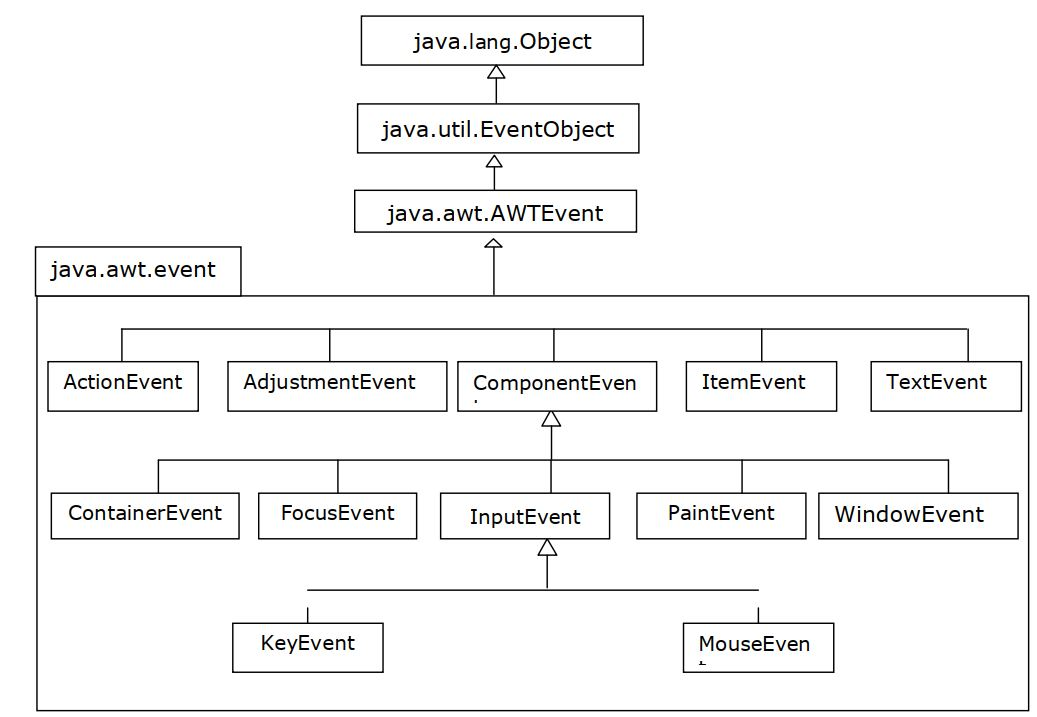
\includegraphics[scale=0.65]{Figures//Hinhtam.jpg}
	\caption{ Các lớp và giao diện của JDBC }\label{hinh3222} 
\end{figure}
Các lớp con của AWTEvent được chia thành hai nhóm:

1. Các lớp mô tả về ngữ nghĩa của các sự kiện,

2. Các lớp sự kiện ở mức thấp
\section{Các lớp sự kiện} 
\subsection{ ActionEvent}
Sự kiện này được phát sinh bởi những hoạt thực hiện trên các thành phần của GUI. Các thành phần gây ra các sự kiện hành động bao gồm:
1 JButton - khi một nút button được khích hoạt,
2 JList - khi một mục trong danh sách được kích hoạt đúp,
3 JmenuItem, JcheckBoxMenu, JradioMenu - khi một mục trong thực đơn
được chọn,
4 JTextField - khi gõ phím ENTER trong trường văn bản (text).
\subsection{ AdjustmentEvent}
Sự kiện này xẩy ra khi ta điều chỉnh (adjustment) giá trị thanh cuốn (JScollBar)
1 Scrollbar - khi thực hiện một lần căn chỉnh trong thanh trượt Scrollbar.
Lớp này có phương thức int getValue(): cho lại giá trị hiện thời được xác định bởi
lần căn chỉnh sau cùng.
\subsection{  ItemEvent}
Các thành phần của GUI gây ra các sự kiện về các mục gồm có:
1 JCheckbox - khi trạng thái của hộp kiểm tra Checkbox thay đổi.
2 CheckboxMenuItem - khi trạng thái của hộp kiểm tra Checkbox ứng với
mục của thực đơn thay đổi.
3 JRadioButton- khi trạng thái của hộp chọn (Option) thay đổi.
4 JList - khi một mục trong danh sách được chọn hoặc bị loại bỏ chọn.
5 JCompoBox - khi một mục trong danh sách được chọn hoặc bị loại bỏ
chọn.
Lớp ItemEvent có phương thức Object getItem(): Cho lại đối tượng được chọn
hay vừa bị bỏ chọn.
\subsection{  TextEvent}
Các thành phần của GUI gây ra các sự kiện về text gồm có:
1 TextArea - khi kết thúc bằng nhấn nút ENTER,
2 TextField - khi kết thúc bằng nhấn nút ENTER
\subsection{  ComponentEvent}
Sự kiện này xuất hiện khi một thành phần bị ẩn đi/hiển ra hoặc thay thay đổi lại
kích thước. Lớp ComponentEvent có phương thức:
Component getComponent()
Cho lại đối tượng tham chiếu kiểu Component.
\subsection{  ContainerEvent}
Sự kiện này xuất hiện khi một thành phần được bổ sung hay bị loại bỏ khỏi
vật chứa (Container).
\subsection{  FocusEvent}
Sự kiện loại này xuất hiện khi một thành phần nhận hoặc mất focus.
\subsection{  KeyEvent}
Lớp KeyEvent là lớp con của lớp trừu tượng InputEvent được sử dụng để
xử lý các sự kiện liên quan đến các phím của bàn phím. Lớp này có các phương
thức:
int getKeyCode()
- Đối với các sự kiện KEY\_PRESSED hoặc KEY\_RELEASED, hàm này được sử
dụng để nhận lại giá trị nguyên tương ứng với mã của phím trên bàn phím.
char getKeyChar()
- Đối với các sự kiện KEY\_PRESSED, hàm này được sử dụng để nhận lại giá trị
nguyên, mã Unicode tương ứng với ký tự của bàn phím.
\subsection{ MouseEvent}
Lớp MouseEvent là lớp con của lớp trừu tượng InputEvent được sử dụng để xử
lý các tín hiệu của chuột. Lớp này có các phương thức:
int getX()
int getY()
Point getPoint()
Các hàm này được sử dụng để nhận lại tọa độ x, y của vị trí liên quan đến
sự kiện do chuột gây ra.
void translatePoint(int dx, int dy)
Hàm translate() được sử dụng để chuyển tọa độ của sự kiện do chuột gây
ra đến (dx, dy).
int getClickCount()
Hàm getClickCount() đếm số lần kích chuột.
\subsection{ PaintEvent}
Sự kiện này xuất hiện khi một thành phần được vẽ lại, thực tế sự kiện này
xẩy ra khi phương thức paint()/ update() được gọi đến.
\subsection{ WindowEvent}
Sự kiện loại này xuất hiện khi thao tác với các Window, chẳng hạn như:
đóng, phóng to, thu nhỏ.. một cửa sổ. Lớp này có phương thức:
Window getWindow()
Hàm này cho lại đối tượng của lớp Window ứng với sự kiện liên quan đến
Window đã xảy ra.